\documentclass[12pt,compress,aspectratio=169]{beamer}

\usetheme{metropolis}
\setbeamersize{text margin left=.5cm,text margin right=.5cm}
  \setbeamertemplate{navigation symbols}{} % suppress nav bar
%  \setbeamercovered{transparent}

\usefonttheme{professionalfonts}
\usepackage{graphicx}
\usepackage{tikz}
\usepackage{amsmath}
\usepackage{mathpazo}
\usepackage{xcolor,colortbl}
%\usepackage{hyperref}
\usepackage{siunitx}

\setmonofont{Ubuntu Mono}
\setlength{\parskip}{0pt}
\renewcommand{\baselinestretch}{1}

\sisetup{
  number-math-rm=\mathnormal,
  inter-unit-product={\ensuremath{\cdot}},
  group-separator={,},
  per-mode=symbol
}

\title{Sound Waves and Music}
\subtitle{Advanced Placement Physics}
\author{Dr.\ Timothy Leung}
\institute{Olympiads School\\Toronto, Ontario, Canada}
\date{Winter/Spring 2020}

\newcommand{\pic}[2]{\includegraphics[width=#1\textwidth]{#2}}
\newcommand{\eq}[2]{\vspace{#1}{\Large\begin{displaymath}#2\end{displaymath}}}

\begin{document}

\begin{frame}
  \titlepage
\end{frame}


\section[Properties]{Properties of Sound}

%\begin{frame}{Sound}
%  \begin{itemize}
%  \item Today we look at one specific application of waves: \textbf{sound}
%  \item Has lots of different applications, including
%    \begin{itemize}
%    \item Aircraft design
%    \item Music
%    \item Noise reduction
%    \end{itemize}
%  \end{itemize}
%
%  \vspace{.2in}\textbf{First, let's learn the lingo\ldots}
%\end{frame}



\begin{frame}{Amplitude: Loudness}
  \begin{center}
    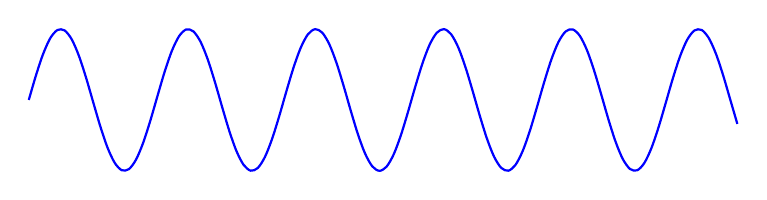
\begin{tikzpicture}[scale=.9]
      \draw[smooth,samples=100,domain=0:10,blue,thick]
      plot({\x},{sin(200*\x)});
    \end{tikzpicture}\\
    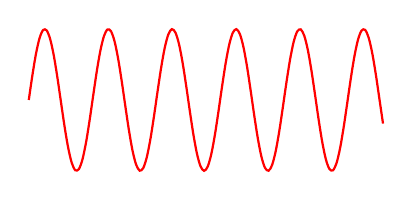
\begin{tikzpicture}[scale=.9]
      \draw[smooth,samples=100,domain=0:5,red,thick]
      plot({\x},{sin(400*\x)});
    \end{tikzpicture}

    \vspace{0.2in}
    \begin{tabular}{cc}
      \rowcolor{pink}
      General waves & Sound Waves \\
      \uncover<1->{\LARGE Amplitude} & {\LARGE Loudness} \\
      & {Perceived \textbf{intensity}} \\
      & {``volume''}
    \end{tabular}

    \begin{itemize}
    \item {\color{blue} Low amplitude}: soft/quiet
    \item {\color{red} High amplitude}: loud
    \item Measured in decibels \si{\decibel}
    \end{itemize}
  \end{center}
\end{frame}



\begin{frame}{Intensity of Sound}
  The energy of a sound wave is proportional to the square of the amplitude
  (pressure difference):

  \eq{-.35in}{ P\propto A^2}

  \vspace{-.2in}The intensity is the power ($P$) divided by the area ($A$) that
  the sound wave passes through:

  \eq{-.25in}{
    \boxed{I=\frac{P}{A}\propto\frac{1}{r^2}}
  }
  
  \vspace{-.1in}When a sound is emitted from a stationary source, the area that
  the wavefront passes through is $A=4\pi r^2$, where $r$ is the distance from
  the source.
\end{frame}



\begin{frame}{Threshold of Hearing}
  The smallest detectable sound intensity is called the
  \textbf{threshold of hearing} $I_0$, defined as:

  \eq{-.2in}{
    I_0=\SI{1e-12}{\watt\per\metre^2}
  }

  While the sound intensity at the \textbf{threshold of pain} can damage a human
  ear:

  \eq{-.2in}{
    I_p=\SI{1}{\watt\per\metre^2}
  }
\end{frame}



\begin{frame}{Threshold of Hearing}
  \begin{center}
    \pic{.6}{earcrv2.png}
  \end{center}
  \begin{itemize}
  \item\vspace{-.15in}The threshold of hearing is actually experimentally
    determined to be about \SI{4e-12}{\watt\per\metre^2} at \SI{1000}{\hertz}.
  \item Maximum sensitivity to sound is \num{3500} to \SI{4000}{\hertz},
    corresponding to the resonance of the auditory canal.
  \end{itemize}
\end{frame}


\begin{frame}{The Decibel}
  The \textbf{decibel} is defined as by the intensity of sound $I$ compared to
  the pre-defined threshold of hearing:
  
  \eq{-.2in}{
    \beta=10\log_{10}\left[\frac{I}{I_0}\right]
  }
  \begin{itemize}
  \item By definition, the threshold of hearing is \SI{0}{dB} while the
    threshold of pain is \SI{120}{dB}.
  \item Humans perceive a doubling of loudness when intensity is increases by a
    factor of \num{10} (an increase of \SI{10}{dB})
  \end{itemize}
\end{frame}

%\begin{frame}{Frequency and Pitch}
%
%  \begin{columns}
%    \column{.5\textwidth}
%    \centering
%    \begin{tabular}{p{1.5in}}
%      \rowcolor{pink}
%      General waves: \\
%      {\LARGE Frequency}
%    \end{tabular}
%
%    \vspace{.3in}{\color{blue} Low frequency} = low pitch
%
%    \begin{tikzpicture}
%      \draw[smooth,samples=40,domain=0:5,blue,thick] plot({\x},{sin(200*\x)});
%    \end{tikzpicture}
%    
%    \column{.5\textwidth}
%    \centering
%    \begin{tabular}{p{1.5in}}
%      \rowcolor{pink}
%      Sound waves:\\
%      {\LARGE Pitch}
%    \end{tabular}
%
%    \vspace{.3in}
%    
%    {\color{red} High frequency} = high pitch
%
%    \begin{tikzpicture}
%      \draw[smooth,samples=80,domain=0:5,red,thick] plot({\x},{sin(500*\x)});
%    \end{tikzpicture}
%
%  \end{columns}
%\end{frame}

\begin{frame}{Frequency and Pitch}
  \begin{columns}
    \column{.65\textwidth}
    \begin{itemize}
    \item Unit for frequency is \textbf{hertz}: \si{\hertz}
      \begin{itemize}
      \item Sound frequencies are usually referred to as its \textbf{pitch}
%      \item In music, the A above the middle C has a standardized frequency of
%        \SI{440}{\hertz}
      \end{itemize}
    \item Audible range for human ears is approximately \SI{20}{\hertz} to
      \SI{20000}{\hertz}
    \item\textbf{Infrasound}: below the audible range
      %Although you can't hear it, you can usually feel the vibrations.
    \item\textbf{Ultrasound}: above the audible range, e.g.
      \begin{itemize}
      \item Dog whistles
      \item Medical ultrasound devices
      \end{itemize}
    \end{itemize}

    \column{.35\textwidth}
    \pic{1}{ultrasound.jpg}\\
    {\footnotesize Medical ultrasound devices usually use frequencies between
    \SI{1}{\mega\hertz} to \SI{20}{\mega\hertz}.\par}
  \end{columns}
\end{frame}


%\begin{frame}{Complexity}
%
%  \begin{center}
%    \begin{tikzpicture}
%      \draw[smooth,samples=100,domain=0:5,blue,thick] plot({\x},{sin(400*\x)});
%    \end{tikzpicture}
%    \begin{tikzpicture}
%      \draw[smooth,samples=100,domain=0:5,red,thick]
%      plot({\x},{sin(300*\x)+0.3*sin(600*\x)+0.2*sin(900*\x)+0.2*(sin(1200*\x)});
%    \end{tikzpicture}
%
%    \vspace{0.2in}
%    \begin{tabular}{cc}
%      \rowcolor{pink}
%      General waves & Sound Waves \\
%      {\LARGE Simple} & {\LARGE Pure} \\
%      {\LARGE Complex}& {\LARGE Rich} \\
%    \end{tabular}
%
%    \begin{itemize}
%    \item {\color{blue} Simple}: e.g.\ sine wave
%    \item {\color{red} Complex}: combination of sine waves
%    \end{itemize}
%  \end{center}
%\end{frame}
%
%
%
%\begin{frame}{Visualizing Waves}
%  We use an \textbf{oscilloscope}:
%  \begin{center}
%    \pic{.35}{images/img_2811.jpg}
%    \pic{.58}{images/oscilloscope1.jpg}
%  \end{center}
%  Learning how to use an oscilloscope is one of the first lessons of every
%  science/engineering student in university physics labs!
%\end{frame}



\begin{frame}{Transfer of Sound Wave in Air}
  \begin{itemize}
  \item Sound wave is a \textbf{longitudinal wave}
  \item Compression and rarefaction (expansion) of the air molecules
  \item Example below: speaker of a stereo system
  \end{itemize}
  \begin{center}
    \pic{.8}{speaker.png}
  \end{center}
\end{frame}



\begin{frame}{Transfer of Sound Wave}
  Example: tuning fork
  \begin{center}
    \pic{.8}{tuningfork.png}
  \end{center}
\end{frame}



\begin{frame}{Transfer of Sound Wave}{Schematic Diagram vs.\ Wave Graph}
  We can also express the amplitude of the sound wave by plotting the change in
  \emph{air pressure}:

  \vspace{-.2in}
  \begin{center}
    \pic{.9}{schematic-vs-graph.png}
  \end{center}
\end{frame}



\section[Transmission]{Transmission of Sound}

\subsection[$v_s$]{Speed of Sound}

\begin{frame}{Speed of Sound in a Gas}
  The speed of sound in a gas (e.g.\ air) depends on temperature and its
  composition:

  \eq{-.4in}{
    \boxed{v_s=\sqrt{\frac{\gamma RT}{M}}}
  }
  \begin{center}
    \begin{tabular}{l|c|c}
      \rowcolor{pink}
      \textbf{Quantity} & \textbf{Symbol} & \textbf{SI Unit} \\ \hline
      Speed of sound           & $v_s$ & \si{\metre\per\second}\\
      Termodynamic temperature & $T$  & \si{\kelvin}\\
      Universal gas constant   & $R$  & \si{\joule\per mol.\kelvin}\\
      Molar mass               & $M$  & \si{\kilo\gram\per mol}\\
      Adiabatic constant ($C_v/C_p$) & $\gamma$  & (no units)
    \end{tabular}
  \end{center}
  For diatomic gases $\gamma=1.4$, and $M=\SI{29e-3}{\kilo\gram/mol}$
\end{frame}



\begin{frame}{Speed of Sound in Air}
  The speed of sound in air near room temperature ($\approx\SI{300}{\kelvin}$)
  can be approximated as function that varies linearly with temperature in
  celsius:
  
  \eq{-.2in}{
    \boxed{v_s=331 + 0.59T_C}
  }
  \begin{center}
    \begin{tabular}{l|c|c}
      \rowcolor{pink}
      \textbf{Quantity} & \textbf{Symbol} & \textbf{SI Unit} \\ \hline
      Speed of sound     & $v_s$ & \si{\metre\per\second}\\
      Temperature of air in celsius & $T_C$ & N/A
    \end{tabular}
  \end{center}
\end{frame}





\begin{frame}{Speed of Sound in Liquids and Solids}
  Speed of sound in a liquid depends on the ``bulk modulus'' $K$ of the liquid,
  and density $\rho$:
      
  \eq{-.35in}{
    v = \sqrt{\frac{K}{\rho}}
  }
   
  Speed of sound in a solid depends on the ``Young's modulus'' $E$ of the solid
  and density $\rho$:

  \eq{-.35in}{
    v = \sqrt{\frac{E}{\rho}}
  }
\end{frame}



\begin{frame}{Speed of Sound in Different Media}
  \begin{center}
    \begin{tabular}{l|c}
      \rowcolor{blue!30}
      \textbf{Material} & \textbf{Speed} (\si{m/s}) \\
      \rowcolor{pink!70}
      \multicolumn{2}{c}{Gases (\SI{0}{\celsius}, \SI{101}{\kilo\pascal})} \\
      Carbon dioxide & $259$ \\
      Oxygen         & $316$ \\
      Air            & $331$ \\
      Helium         & $965$ \\
      \rowcolor{pink!70}
      \multicolumn{2}{c}{Liquids (\SI{20}{\celsius})} \\
      Ethanol        & $1162$ \\
      Fresh water    & $1482$ \\
      Seawater (depends on depth and salinity) & $1440-1500$ \\
      \rowcolor{pink!70}
      \multicolumn{2}{c}{Solids} \\
      Copper         & $5010$ \\
      Glass (heat-resistant) & $5640$ \\
      Steel          & $5960$
    \end{tabular}
  \end{center}
\end{frame}



\subsection[$M$]{Mach Number}

\begin{frame}{Mach Number}
  Speeds close to the speed of sound is often expressed in terms of its ratio
  to the speed of sound. This is called the \textbf{Mach number} ($M$):
  
  \eq{-.2in}{
    \boxed{M=\frac{v}{v_s}}
  }
  \begin{center}
    \begin{tabular}{l|c|c}
      \rowcolor{pink}
      \textbf{Quantity} & \textbf{Symbol} & \textbf{SI Unit} \\ \hline
      Mach number          & $M$   & no units \\
      Speed of the object  & $v$   & \si{\metre\per\second} \\
      Local speed of sound & $v_s$ & \si{\metre\per\second}
    \end{tabular}
  \end{center}
  \begin{itemize}
  \item When an object is travelling at $M<1$, it is travelling at a
    \emph{subsonic} speed
  \item When an object is travelling at $M>1$, it is travelling at a
    \emph{supersonic} speed
  \end{itemize}
\end{frame}



\begin{frame}{Sound from a Stationary Source}
  When a sound is emitted from a stationary point source, the sound wave moves
  radially outward from the origin:
  \begin{center}
    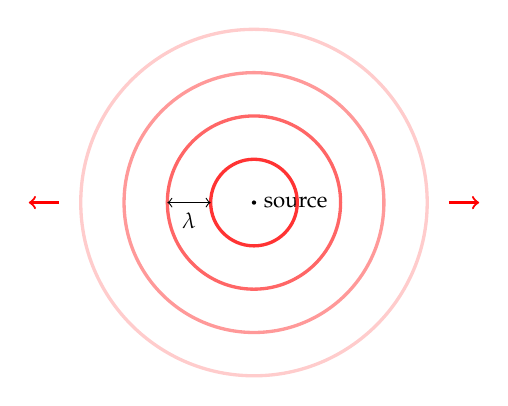
\begin{tikzpicture}[scale=.55]
      \fill[black](0,0) circle(.05) node[right]{\footnotesize source};
      \begin{scope}[very thick]
        \uncover<2->{ \draw[red!80](0,0) circle(1); }
        \uncover<3->{ \draw[red!60](0,0) circle(2); }
        \uncover<4->{ \draw[red!40](0,0) circle(3); }
        \uncover<5->{ \draw[red!20](0,0) circle(4); }
      \end{scope}
      \uncover<5->{
        \draw[<->](-1,0)--(-2,0) node[midway,below]{\footnotesize $\lambda$};
        \draw[thick,->,red](4.5,0)--(5.2,0);
        \draw[thick,->,red](-4.5,0)--(-5.2,0);
      }
    \end{tikzpicture}
    \begin{itemize}
    \item Sound intensity (amplitude) drops farther away from the source
    \item All points hear the same wavelength (and frequency) of sound
    \end{itemize}
  \end{center}
\end{frame}



\subsection[Doppler]{Doppler Effect}

\begin{frame}{Sound from a Moving Source}
  When sound is emitted from a \emph{moving} source, the diagram looks
  different. In this case, the sound source is moving to the right, from $1$ to
  $4$:
  \vspace{.2in}
  \begin{columns}
    \column{.3\textwidth}
    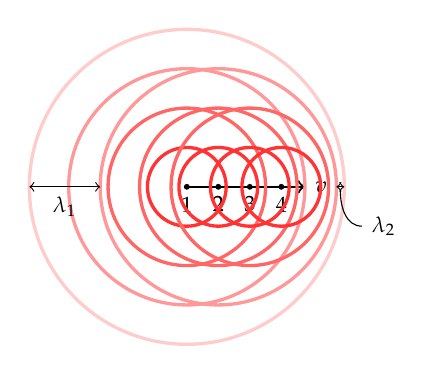
\begin{tikzpicture}[scale=.5]
      \fill ( 0,0) circle(.075) node[below]{\footnotesize $1$};
      \uncover<2->{ \fill (.8,0) circle(.075) node[below]{\footnotesize $2$}; }
      \uncover<3->{ \fill(1.6,0) circle(.075) node[below]{\footnotesize $3$}; }
      \uncover<4->{ \fill(2.4,0) circle(.075) node[below]{\footnotesize $4$}; }
      \draw[thick,->](0,0)--(3,0) node[pos=1,right]{\footnotesize $v$};
      \begin{scope}[very thick]
        \uncover<2>{
          \draw[red!80](0,0) circle(1);
        }
        \uncover<3>{
          \draw[red!60](0,0) circle(2);
          \draw[red!80](.8,0)circle(1);
        }
        \uncover<4>{
          \draw[red!40]  (0,0) circle(3);
          \draw[red!60] (.8,0) circle(2);
          \draw[red!80](1.6,0) circle(1);
        }
        \uncover<5>{
          \draw[red!20](  0,0) circle(4);
          \draw[red!40]( .8,0) circle(3);
          \draw[red!60](1.6,0) circle(2);
          \draw[red!80](2.4,0) circle(1);
        }
      \end{scope}
      \uncover<5->{
        \draw[<->](-4,0)--(-2.2,0)
        node[midway,below]{\footnotesize $\lambda_1$};
        \draw[<->](4,0)--(3.8,0);
        \node (a) at (5,-1) {\footnotesize $\lambda_2$};
        \draw(3.9,-.1) to[out=270,in=180] (a);
      }
    \end{tikzpicture}
      
    \column{.7\textwidth}
    \uncover<5>{
      \begin{itemize}
      \item When the source is moving \emph{towards you}, the wavelength
        $\lambda_2$ decreases, and the apparent frequency increases.
      \item When the source is moving \emph{away from you}, the wavelength
        $\lambda_1$ increases, and the aparent frequency decreases.
      \end{itemize}

      \vspace{.2in}This is called the \textbf{Doppler effect}.
    }
  \end{columns}
\end{frame}



\begin{frame}{Doppler Effect}
  We all experience Doppler effect every time an ambulance speeds by us with
  its sirens on.
  \begin{center}
    \pic{.6}{toronto-ambulance.jpg}
  \end{center}
  When it is moving towards us, the pitch of the siren is high, but the moment
  it passes us, the pitch decreases.
\end{frame}



\begin{frame}{Doppler Effect}
  When a wave source is moving at a speed $v_{\textrm{src}}$ and an observing is
  moving at observer $v_{\textrm{ob}}$, the perceived frequency is shifted:

  \eq{-.2in}{
    \boxed{f'=\frac{v_s\pm v_{\textrm{ob}}}{v_s\mp v_{\textrm{src}}}f}
  }
  \begin{center}
    \begin{tabular}{l|c|c}
      \rowcolor{pink}
      \textbf{Quantity} & \textbf{Symbol} & \textbf{SI Unit} \\ \hline
      Apparent frequency  & $f'$   & \si{\hertz} \\
      Actual frequency    & $f$    & \si{\hertz} \\
      Speed of sound      & $v_s$ & \si{\metre\per\second}\\
      Speed of source & $v_{\textrm{src}}$ & \si{\metre\per\second}\\
      Speed of observer & $v_{\textrm{ob}}$ & \si{\metre\per\second}
    \end{tabular}
  \end{center}
  %The Doppler effect equation applies to all types of waves, including sound
  %waves \emph{and} electromagnetic waves.
\end{frame}


\subsection{Sonic Boom}

\begin{frame}{Sound Source at Sonic Speed}
  Doppler effect is even more interesting is when sound source is moving at the
  speed of sound ($M=1$):

  \vspace{.2in}\begin{columns}
    \column{.3\textwidth}
    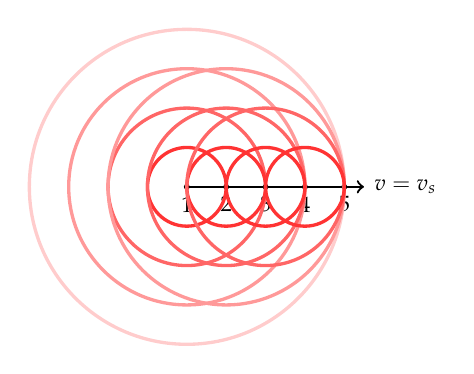
\begin{tikzpicture}[scale=.5]
      \draw[->,thick](0,0)--(4.5,0) node[pos=1,right]{\footnotesize $v=v_s$};
      \fill(0,0) circle(.075) node[below]{\footnotesize $1$};
      \uncover<2->{ \fill(1,0) circle(.075) node[below]{\footnotesize $2$}; }
      \uncover<3->{ \fill(2,0) circle(.075) node[below]{\footnotesize $3$}; }
      \uncover<4->{ \fill(3,0) circle(.075) node[below]{\footnotesize $4$}; }
      \uncover<5->{ \fill(4,0) circle(.075) node[below]{\footnotesize $5$}; }

      \begin{scope}[very thick]
        \uncover<2>{
          \draw[red!80](0,0) circle(1);
        }
        \uncover<3>{
          \draw[red!60](0,0) circle(2);
          \draw[red!80](1,0)circle(1);
        }
        \uncover<4>{
          \draw[red!40](0,0) circle(3);
          \draw[red!60](1,0) circle(2);
          \draw[red!80](2,0) circle(1);
        }
        \uncover<5>{
          \draw[red!20](0,0) circle(4);
          \draw[red!40](1,0) circle(3);
          \draw[red!60](2,0) circle(2);
          \draw[red!80](3,0) circle(1);
        } 
      \end{scope}
    \end{tikzpicture}
      
    \column{.7\textwidth}
    \uncover<5>{
      \begin{itemize}
      \item The wavefronts (crests) from all the waves are bunched up just in
        front of the source
      \item Since sound wave is a pressure wave, right in front of the sound
        source, there is a large change in pressure (called a shock wave)
      \item When the shock passes an observer, an loud bang can be heard (aka
        \textbf{sonic boom})
    }
    \end{itemize}
  \end{columns}
\end{frame}



\begin{frame}{Sound from a Supersonic Source}
  When sound source is moving at $M>1$, it out runs the sound that it makes:
  \begin{columns}
    \column{.47\textwidth}
    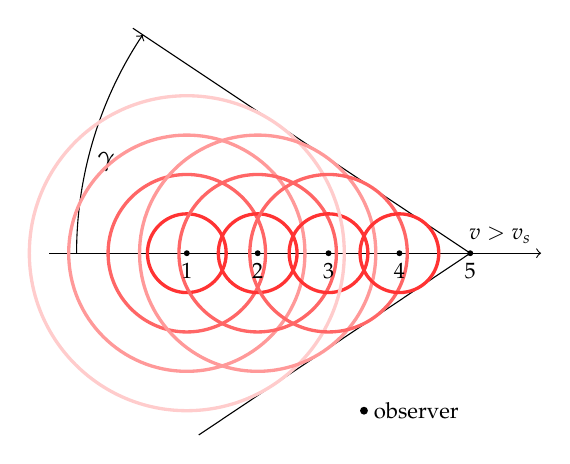
\begin{tikzpicture}[scale=.5]
      
      \draw[->](-3.5,0)--(9,0) node[pos=1,above left]{\footnotesize $v>v_s$};
      \uncover<5>{
        \draw[rotate around={213.8:(7.2,0)}](7.2,0)--(15.5,0);
        \draw[rotate around={146.3:(7.2,0)}](7.2,0)--(17.5,0);
        \draw[->](-2.8,0) arc(180:146.3:10) node[pos=.4,right]{$\gamma$};
        \fill[black](4.5,-4) circle(.1) node[right]{\footnotesize observer};
      }
      \begin{scope}[very thick]
        \uncover<2>{
          \draw[red!80](0,0) circle(1);
        }
        \uncover<3>{
          \draw[red!60](0,0) circle(2);
          \draw[red!80](1.8,0)circle(1);
        }
        \uncover<4>{
          \draw[red!40](0,0) circle(3);
          \draw[red!60](1.8,0) circle(2);
          \draw[red!80](3.6,0) circle(1);
        }
        \uncover<5>{
          \draw[red!20](0,0) circle(4);
          \draw[red!40](1.8,0) circle(3);
          \draw[red!60](3.6,0) circle(2);
          \draw[red!80](5.4,0) circle(1);
        } 
      \end{scope}
      \fill(0,0) circle(.075) node[below]{\footnotesize $1$};
      \uncover<2->{ \fill(1.8,0) circle(.075) node[below]{\footnotesize $2$}; }
      \uncover<3->{ \fill(3.6,0) circle(.075) node[below]{\footnotesize $3$}; }
      \uncover<4->{ \fill(5.4,0) circle(.075) node[below]{\footnotesize $4$}; }
      \uncover<5->{ \fill(7.2,0) circle(.075) node[below]{\footnotesize $5$}; }
    \end{tikzpicture}
      
    \column{.53\textwidth}
    \uncover<5>{
      An \emph{oblique shock} is formed at an angle (called the
      \textbf{Mach angle}) given by:
      
      \eq{-.1in}{
        \gamma=\sin^{-1}\left(\frac{1}{M}\right)
      }

      An observer does not hear the sound source until it has gone past!
    }
  \end{columns}
\end{frame}



\begin{frame}{Bullet in Supersonic Flight}
  Generating a shock doesn't require an actual sound source. Any object
  moving through air creates a pressure disturbance. This is a
  \SI{7.62}{\milli\metre} NATO bullet in supersonic flight.
  \begin{center}
    \pic{.35}{bullet2.jpg}
  \end{center}
  The flow around this bullet is taken inside a \emph{shock tube} that
  generates a short burst of supersonic flow. A high-speed camera is used to
  take the photo.
\end{frame}



\begin{frame}{Duck in Water}{No sonic booms here}
  A similar shock behaviour is observed when the duck swims in water, because
  the duck swims faster than the speed of the water wave, it also creates a
  cone shape.
  \begin{center}
    \pic{.5}{duck.jpg}
  \end{center}

\end{frame}



%\begin{frame}{Transonic Speed}
%  For aircraft designers (like Tim), the most flow is at \emph{transonic}
%  speeds ($0.6<M<1$) where the flow around the aircraft is a mixture of
%  supersonic and subsonic flow.
%\end{frame}



\section{Wave Interference}

\subsection{Beat Frequency}

\begin{frame}{Visualizing Beat Frequency}
  We plot two waves moving in the same medium, but with slightly different
  frequencies (Think of them as the two musical instruments playing two slightly
  different pitch)
  \begin{center}
    \vspace{-.1in}
    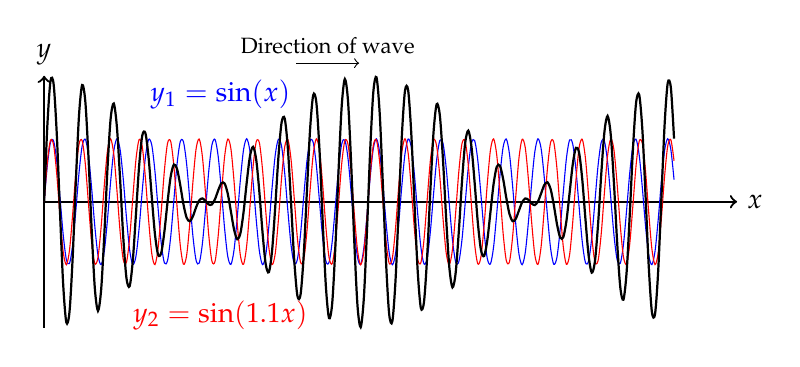
\begin{tikzpicture}[scale=.8]
      \draw[->,thick](0,0) --(11,0) node[pos=1,right] {$x$};
      \draw[->,thick](0,-2)-- (0,2) node[pos=1,above] {$y$};
      \draw[->](4,2.2)--(5,2.2)
      node[midway,above]{\footnotesize Direction of wave};
      \uncover<1,3->{
        \node at (2.8,1.7) {$\color{blue}{y_1=\sin(x)}$};
        \draw[blue,smooth,samples=200,domain=0:10] plot({\x},{sin(700*\x)});
      }
      \uncover<2->{
        \node at (2.8,-1.8) {$\color{red}{y_2=\sin(1.1x)}$};
        \draw[smooth,samples=200,domain=0:10,red] plot({\x},{sin(770*\x)});
      }
      \uncover<4>{
        \draw[smooth,samples=200,domain=0:10,thick]
        plot({\x},{sin(700*\x)+sin(770*\x)});
      }
    \end{tikzpicture}
  \end{center}
  \uncover<4->{
    The thick black line shows the sum of the waves: $y=\sin(x)+\sin(1.1x)$
  }
\end{frame}



\begin{frame}{Beat Frequency}
  The \textbf{beat frequency} is the absolute value of the difference of the
  frequencies of the two component waves:

  \eq{-.2in}{
    \boxed{f_\mathrm{beat}=|f_2-f_1|}
  }
  \vspace{-.1in}
  \begin{center}
    \begin{tabular}{l|c|c}
      \rowcolor{pink}
      \textbf{Quantity} & \textbf{Symbol} & \textbf{SI Unit} \\ \hline
      Beat frequency     & $f_\mathrm{beat}$   & \si{\hertz} \\
      Frequency of 1st component wave & $f_1$ & \si{\hertz} \\
      Frequency of 2nd component wave & $f_2$ & \si{\hertz}
    \end{tabular}
  \end{center}
\end{frame}



\section[Music]{Physics of Music}

\begin{frame}{Music vs.\ Noise}
  Difference between \emph{noise} and \emph{music} is often difficult to
  distinguish. Generally, the concept of music is based on:
  \begin{itemize}
  \item Organized combinations of different frequencies
  \item Harmonics of dominated frequencies, which are
  \item Whole-number multiples of the lowest (fundamental) frequency
  \end{itemize}
\end{frame}



%\begin{frame}{Musical Instruments}
%  \begin{itemize}
%  \item Question: A violin sounds different from a trumpet. Why?
%  \item Answer: Because the waves from different instruments are different.
%  \item Question: Buy why do waves with different shapes sound differently?
%  \item Answer: Let's ask Joseph Fourier!
%  \end{itemize}
%\end{frame}
%
%
\subsection{Harmonics}

\begin{frame}{Musical Instruments}
  When a musical instrument produces a sound at a certain frequency, it also
  produces higher frequency sounds
  \begin{itemize}
  \item The higher frequency sounds are \emph{whole-number multiples} of the
    lowest frequency
  \item e.g.\ a violin playing at \SI{440}{\hertz} produces sound waves at

    \vspace{-.1in}\begin{displaymath}
      \SI{440}{\hertz}, \SI{880}{\hertz}, \SI{1320}{\hertz},
      \SI{1760}{\hertz}, \SI{2200}{\hertz}, \SI{2640}{\hertz}\ldots
    \end{displaymath}
  \item Generally, the higher the frequency, the smaller the amplitude
  \item The overall quality of the sound is the sum of all the waves.
    This is why a violin and a trumpet can both play the same note, but sounding
    different
  \end{itemize}
\end{frame}



%\begin{frame}{Fourier Series}
%  French mathematician Joseph Fourier discovered that \emph{all} periodic
%  functions are combinations of $\sin$ and/or $\cos$ functions, like this:
%%  \begin{columns}
%%    \column{0.3\textwidth}
%%    \begin{center}
%%      \pic{1}{images/Fourier2.jpg}\\
%%      {\footnotesize
%%        French mathematician
%%        Joseph Fourier
%%      }
%%    \end{center}
%%    \column{0.7\textwidth}
%%    \begin{itemize}
%%    \item Every periodic function (i.e.\ wave) can be written as a fundamental
%%      frequency plus its harmonics
%  %    \item In math, we write:
%
%  \vspace{-.35in}{\large
%    \begin{displaymath}
%      f(x)=a_1\sin(x)+a_2\sin(2x)+a_3\sin(3x)+\ldots
%      =\sum_{n=1}^{\infty}a_n\sin(nx)
%    \end{displaymath}
%  }
%
%  \vspace{-.15in}Think of each $\sin$ function as a wave with related
%  wavelengths and frequencies
%  \begin{center}
%    \vspace{-.15in}
%    \begin{tikzpicture}[scale=.9]
%      \draw[->,thick](0,0) --(3,0);
%      \draw[->](1,1.3)--(1.5,1.3) node[midway,above]{\footnotesize $v$};
%      \draw[thick,blue,smooth,samples=60,domain=0:2.8] plot({\x},{sin(200*\x)});
%    \end{tikzpicture}
%    \hspace{.15in}
%    \begin{tikzpicture}[scale=.9]
%      \draw[->,thick](0,0) --(3,0);
%      \draw[->](1,1.3)--(1.5,1.3) node[midway,above]{\footnotesize $v$};
%      \draw[thick,red,smooth,samples=60,domain=0:2.8] plot({\x},{sin(400*\x)});
%    \end{tikzpicture}
%    \hspace{.15in}
%    \begin{tikzpicture}[scale=.9]
%      \draw[->,thick](0,0) --(3,0);
%      \draw[->](1,1.3)--(1.5,1.3) node[midway,above]{\footnotesize $v$};
%      \draw[thick,green,smooth,samples=60,domain=0:2.8]
%      plot({\x},{sin(600*\x)});
%    \end{tikzpicture}
%    \hspace{.15in}$\cdots$
%  \end{center}
%  
%  \vspace{-.1in}The coefficients $a_n$ are the amplitudes of the waves (they can
%  be zero)
%\end{frame}



\begin{frame}{Harmonic Frequencies}
  \begin{center}
    \vspace{-.3in}
    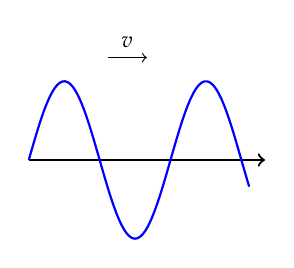
\begin{tikzpicture}
      \draw[->,thick](0,0) --(3,0);
      \draw[->](1,1.3)--(1.5,1.3) node[midway,above]{\footnotesize $v$};
      \draw[thick,blue,smooth,samples=80,domain=0:2.8] plot({\x},{sin(200*\x)});
    \end{tikzpicture}
    \hspace{.15in}
    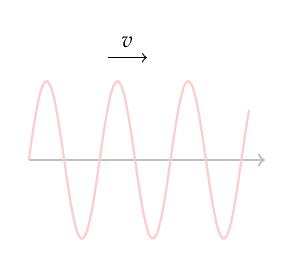
\begin{tikzpicture}
      \draw[->,gray!50,thick](0,0) --(3,0);
      \draw[->](1,1.3)--(1.5,1.3) node[midway,above]{\footnotesize $v$};
      \draw[thick,red!20,smooth,samples=80,domain=0:2.8] plot({\x},{sin(400*\x)});
    \end{tikzpicture}
    \hspace{.15in}
    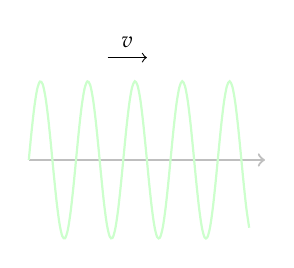
\begin{tikzpicture}
      \draw[->,gray!50,thick](0,0) --(3,0);
      \draw[->](1,1.3)--(1.5,1.3) node[midway,above]{\footnotesize $v$};
      \draw[thick,green!20,smooth,samples=80,domain=0:2.8]
      plot({\x},{sin(600*\x)});
    \end{tikzpicture}
  \end{center}

  \vspace{-.2in}
  The sound wave with the longest wavelength and lowest frequency is:
  \begin{itemize}
  \item\textbf{fundamental frequency}, which is also called
  \item\emph{first harmonic}
  \item\emph{first partial}
  \end{itemize}
  Generally, when a musical instrument produces a sound, the fundamental
  frequency is the one that is ``heard''
\end{frame}



\begin{frame}{Harmonic Frequencies}
  \begin{center}
    \vspace{-.3in}
    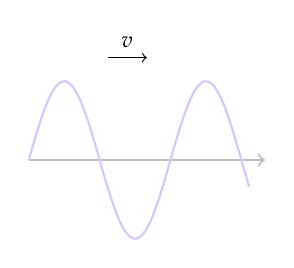
\begin{tikzpicture}
      \draw[->,gray!50,thick](0,0) --(3,0);
      \draw[->](1,1.3)--(1.5,1.3) node[midway,above]{\footnotesize $v$};
      \draw[thick,blue!20,smooth,samples=80,domain=0:2.8] plot({\x},{sin(200*\x)});
    \end{tikzpicture}
    \hspace{.15in}
    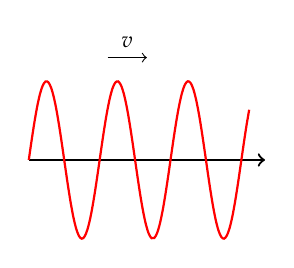
\begin{tikzpicture}
      \draw[->,thick](0,0) --(3,0);
      \draw[->](1,1.3)--(1.5,1.3) node[midway,above]{\footnotesize $v$};
      \draw[thick,red,smooth,samples=80,domain=0:2.8] plot({\x},{sin(400*\x)});
    \end{tikzpicture}
    \hspace{.15in}
    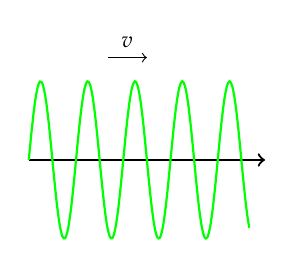
\begin{tikzpicture}
      \draw[->,thick](0,0) --(3,0);
      \draw[->](1,1.3)--(1.5,1.3) node[midway,above]{\footnotesize $v$};
      \draw[thick,green,smooth,samples=80,domain=0:2.8]
      plot({\x},{sin(600*\x)});
    \end{tikzpicture}
  \end{center}
  A second wave has half the wavelength and twice the frequency. It's called:
  \begin{itemize}
  \item\emph{second harmonic}
  \item\emph{second partial}
  \item\emph{first overtone}
  \end{itemize}
  From there we have the third, fourth, fifth\ldots harmonics
\end{frame}



\begin{frame}{Harmonic Frequencies}
  Whole-number multiples of the fundamental frequency $f_1$ are its
  \textbf{harmonic frequencies}, i.e.\ the $n$-th harmonic is:

  \eq{-.2in}{
    \boxed{f_{h,n}=nf_1}\quad\quad n\geq 1
  }
  
  \textbf{Pro-tip:} Different physics and musical traditions use slightly
  different terminologies when talking about ``harmonics''. The words
  \emph{overtones} and \emph{partials} are often use, not always correctly. If
  you hear these terms, clarify with the person what they mean.
\end{frame}



\begin{frame}{Different Musical Instruments}
  Waveforms from different musical instruments at \SI{440}{\hertz}:
  \begin{center}
    \pic{.65}{F_InstrumentWaves.png}
  \end{center}
  The graph on the right correspond to the amplitudes at different frequencies.
  Note the peaks at regular intervals. Those are the harmonic frequencies.
\end{frame}




%\begin{frame}{Making a Square Wave with Sine Waves}
%  \begin{columns}
%    
%    \column{.6\textwidth}
%    \centering
%    \begin{tikzpicture}[xscale=.013,yscale=2.3]
%      \draw[->](0,0)--(380,0) node[pos=1,right]{$x$};
%      \uncover<1>{
%        \draw[samples=60,domain=0:360,red,very thick]plot({\x},{sin(\x)});
%      }
%      \uncover<2>{
%        \draw[samples=80,domain=0:360,orange,very thick]
%        plot({\x},{sin(\x)+1/3*sin(3*\x)});
%      }
%      \uncover<3>{
%        \draw[samples=100,domain=0:360,yellow,very thick]
%        plot({\x},{sin(\x)+1/3*sin(3*\x)+1/5*sin(5*\x)});
%      }
%      \uncover<4>{
%        \draw[smooth,samples=140,domain=0:360,green,very thick]
%        plot({\x},{sin(\x)+1/3*sin(3*\x)+1/5*sin(5*\x)+1/7*sin(7*\x)});
%      }
%      \uncover<5>{
%        \draw[smooth,samples=160,domain=0:360,blue,very thick]
%        plot({\x},
%        {sin(\x)+1/3*sin(3*\x)+1/5*sin(5*\x)+1/7*sin(7*\x)+1/9*sin(9*\x)});
%      }
%      \uncover<6>{
%        \draw[smooth,samples=160,domain=0:360,purple,very thick]
%        plot({\x},
%        {sin(\x)+1/3*sin(3*\x)+1/5*sin(5*\x)+1/7*sin(7*\x)+1/9*sin(9*\x)+
%          1/11*sin(11*\x)});
%      }
%      \uncover<7>{
%        \draw[smooth,samples=200,domain=0:360,very thick]
%        plot({\x},
%        {sin(\x)+1/3*sin(3*\x)+1/5*sin(5*\x)+1/7*sin(7*\x)+1/9*sin(9*\x)+
%          1/11*sin(11*\x)+
%          1/13*sin(13*\x)});
%      }
%      \uncover<8>{
%        \draw[smooth,samples=200,domain=0:360,very thick]
%        plot({\x},
%        {sin(\x)+1/3*sin(3*\x)+1/5*sin(5*\x)+1/7*sin(7*\x)+1/9*sin(9*\x)+
%          1/11*sin(11*\x)+
%          1/13*sin(13*\x)+
%          1/15*sin(15*\x)});
%      }
%      \uncover<9>{
%        \draw[smooth,samples=350,domain=0:360,very thick]
%        plot({\x},
%        {sin(\x)+1/3*sin(3*\x)+1/5*sin(5*\x)+1/7*sin(7*\x)+1/9*sin(9*\x)+
%          1/11*sin(11*\x)+ 1/13*sin(13*\x)+ 1/15*sin(15*\x)+ 1/17*sin(17*\x)+
%          1/19*sin(19*\x)+
%          1/21*sin(21*\x)+ 1/23*sin(23*\x)+ 1/25*sin(25*\x)+ 1/27*sin(27*\x)+
%          1/29*sin(29*\x)+
%          1/31*sin(31*\x)+ 1/33*sin(33*\x)+ 1/35*sin(35*\x)+ 1/17*sin(37*\x)+
%          1/39*sin(39*\x)});
%      }
%    \end{tikzpicture}
%
%    \column{.35\textwidth}
%    \uncover<1->{
%      \begin{tikzpicture}[xscale=.006,yscale=.5]
%        \draw(0,0)--(380,0) node[pos=1,right]{\color{red}$f_1=\sin(x)$};
%        \draw[samples=60,domain=0:360,red,very thick] plot({\x},{sin(\x)});
%      \end{tikzpicture}
%    }
%    \uncover<2->{
%      \begin{tikzpicture}[xscale=.006,yscale=.5]
%        \draw(0,0)--(380,0) node[pos=1,right]
%             {\color{orange}$f_1=\frac{1}{3}\sin(3x)$};
%        \draw[samples=60,domain=0:360,orange,very thick] plot({\x},{sin(3*\x)});
%      \end{tikzpicture}
%    }
%    \uncover<3->{
%      \begin{tikzpicture}[xscale=.006,yscale=.5]
%        \draw(0,0)--(380,0) node[pos=1,right]
%             {\color{yellow}$f_1=\frac{1}{5}\sin(5x)$};
%        \draw[samples=80,domain=0:360,yellow,very thick] plot({\x},{sin(5*\x)});
%      \end{tikzpicture}
%    }
%    \uncover<4->{
%      \begin{tikzpicture}[xscale=.006,yscale=.5]
%        \draw(0,0)--(380,0) node[pos=1,right]
%             {\color{green}$f_1=\frac{1}{7}\sin(7x)$};
%        \draw[samples=200,domain=0:360,green,very thick] plot({\x},{sin(7*\x)});
%      \end{tikzpicture}
%    }
%    \uncover<5->{
%      \begin{tikzpicture}[xscale=.006,yscale=.5]
%        \draw(0,0)--(380,0) node[pos=1,right]
%             {\color{green}$f_1=\frac{1}{9}\sin(9x)$};
%        \draw[samples=200,domain=0:360,blue,very thick] plot({\x},{sin(9*\x)});
%      \end{tikzpicture}
%    }
%  \end{columns}
%\end{frame}



\begin{frame}{Fourier Analysis and Synthesis}
  \begin{center}
    \pic{.6}{Fourier-xform.png}
  \end{center}
\end{frame}



\begin{frame}{Your Piano is \textbf{Always} Out of Tune!}
  \begin{itemize}
  \item The concept of harmonic frequencies is the reason why some musical
    instruments will never play well in harmony (e.g.\ pianos, modern organs).
  \item \textbf{Example:} Find all the harmonics of a fundamental frequency of
    \SI{110}{\hertz} and then compare them to the values on the table.
  \end{itemize}
  \begin{center}
    \pic{.6}{fundamental_freqs.png}
  \end{center}
\end{frame}



\subsection[Strings]{Standing Waves on Strings}

\begin{frame}{Standing Waves On a String}
  \begin{itemize}
  \item A ``vibrating'' string is actually a standing wave on a string
  \item Both ends of the string are nodes
  \item As the string vibrates, the air around it vibrates at the same frequency
  \item The vibration travels as a sound wave towards your ears
  \item Examples:
    \begin{itemize}
    \item Plucking a guitar or violin string
    \item Hitting a key on a piano/harpsichord
    \end{itemize}
  \end{itemize}

%  \vspace{0.5in}{\footnotesize
%    \textbf{Pro-tip:} Want to sound super smart? Plucking a violin string is
%    called \emph{pizzicato} in Italian.\par
%  }
\end{frame}



\begin{frame}{Standing Waves On a String of Length $L$}
  \textbf{Resonance frequencies} are frequencies where a standing wave can be
  created. The first resonance (fundamental) frequency at occurs when
  $\lambda=2L$:
  \begin{center}
    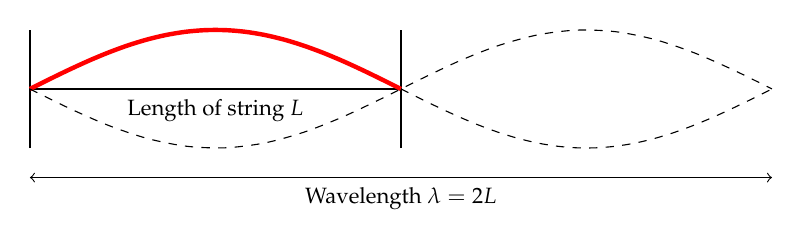
\begin{tikzpicture}[scale=1.5]
      \draw[thick](0,0) -- (pi,0)
      node[midway,below]{\footnotesize Length of string $L$};
      \draw[thick](0,-.5) --(0,.5);
      \draw[thick](pi,-.5)--(pi,.5);
      \draw[smooth,samples=20,domain=0:pi,red,ultra thick]
      plot({\x},{0.5*sin(180/pi*\x)});
      \draw[smooth,samples=20,domain=pi:2*pi,dashed]
      plot({\x},{0.5*sin(180/pi*\x)});
      \draw[smooth,samples=20,domain=0:2*pi,dashed]
      plot({\x},{-.5*sin(180/pi*\x)});
      \draw[<->](0,-.75)--(2*pi,-.75)
      node[midway,below]{\footnotesize Wavelength $\lambda=2L$};
    \end{tikzpicture}
  \end{center}
  
  \vspace{-.1in}The fundamental frequency is based on the speed of the
  travelling wave along the string $v_\mathrm{str}$:

  \eq{-.3in}{
    \boxed{
      f_{r,1}
      =\frac{v_\mathrm{str}}{\lambda}=\frac{v_\mathrm{str}}{2L}}
  }
\end{frame}



\begin{frame}{Standing Waves On a String of Length $L$}
  A second resonance frequency occurs when $L=\lambda$:

  \vspace{-.2in}\begin{columns}
    \column{.45\textwidth}
    \centering
    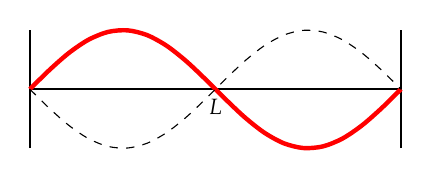
\begin{tikzpicture}[scale=1.5]
      \draw[thick](0,0)--(pi,0) node[midway,below]{\footnotesize $L$};
      \draw[thick](0,-.5)--(0,.5);
      \draw[thick](pi,-.5)--(pi,.5);
      \draw[smooth,samples=20,domain=0:pi,red,ultra thick]
      plot({\x},{.5*sin(360/pi*\x)});
      \draw[smooth,samples=20,domain=0:pi,dashed]
      plot({\x},{-.5*sin(360/pi*\x)});
    \end{tikzpicture}
    
    \column{.55\textwidth}
    
    \eq{-.01in}{
      f_{r,2}=
      \frac{v_\mathrm{str}}{\lambda}=\frac{v_\mathrm{str}}{L}=2f_{r,1}
    }
  \end{columns}

  And a third resonance frequency occurs at
  $\displaystyle L=\frac{3}{2}\lambda$:

  \vspace{-.2in}
  \begin{columns}
    \column{.45\textwidth}
    \centering
    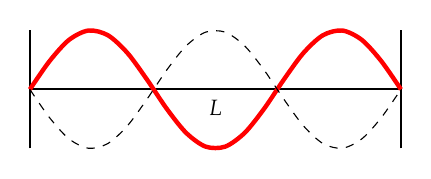
\begin{tikzpicture}[scale=1.5]
      \draw[thick](0,0)--(pi,0) node[midway,below]{\footnotesize $L$};
      \draw[thick](0,-.5)--(0,.5);
      \draw[thick](pi,-.5)--(pi,.5);
      \draw[smooth,samples=20,domain=0:pi,red,ultra thick]
      plot({\x},{.5*sin(540/pi*\x)});
      \draw[smooth,samples=20,domain=0:pi,dashed]
      plot({\x},{-.5*sin(540/pi*\x)});
    \end{tikzpicture}
    
    \column{.55\textwidth}
      
    \eq{-.01in}{
      f_{r,3}=\frac{3v_\mathrm{str}}{2L}=3f_{r,1}
    }
  \end{columns}
\end{frame}



\begin{frame}{Standing Waves On a String of Length $L$}
  In fact, the $n$-th resonance frequency of a wave on string is:

  \eq{-.2in}{
    \boxed{f_{r,n}=nf_{r,1}}\quad
    \text{\normalsize (standing wave on string)}
  }
  \begin{itemize}
  \item where the fundamental frequency is
    
    \eq{-.2in}{
      \boxed{f_{r,1}=\frac{v_{\textrm{str}}}{2L}}
    }
  \item $n$ is a whole-number multiple
  \item This equation is \emph{identical} to the equation for harmonic
    frequencies, meaning that on a string, every harmonic is a resonance
    frequency
  \item A vibrating string is said to have a ``full set of harmonics''
  \end{itemize}
\end{frame}



%\begin{frame}{Standing Wave on a String: The Violin}
%  \begin{columns}
%    \column{0.45\textwidth}
%    \pic{1}{images/String2-700x420.png}\\
%    Violinist Joshua Bell
%
%    {\tiny (It's almost next to impossible to find a decent photo of someone
%      playing the violin. So many bad photos out there\ldots)
%    }
%    \column{0.55\textwidth}
%    \begin{itemize}
%    \item The friction between the string and the hair of the bow (coated in
%      \emph{rosin} pulls the string
%    \item The tension on the string overcomes the friction and the string begins
%      to vibrate (i.e.\ standing wave-pattern begins)
%    \item Since the initial shape of the string is not a perfect sine wave,
%      the actual wave created is a combination of the fundamental and all the
%      resonance frequencies
%    \end{itemize}
%  \end{columns}
%\end{frame}



%\begin{frame}{Standing Wave on a String: The Violin}
%    \begin{itemize}
%    \item We can actually see the amplitudes of all the harmonics on the
%      violin:
%      \begin{center}
%        \pic{0.55}{images/violin_sprectrum.png}
%      \end{center}
%    \item In general, the higher the harmonics,
%      the smaller the amplitudes, but instruments like violin \& flute have
%      very high relative amplitudes at higher harmonics
%    \end{itemize}
%\end{frame}
%


\subsection[Pipes]{Standing Waves in Pipes}

\begin{frame}{Standing Waves in Closed Pipes}
  The same standing-wave patterns (nodes on both ends of the pipe) can be found
  on pipes that have both ends closed:

  \begin{center}
    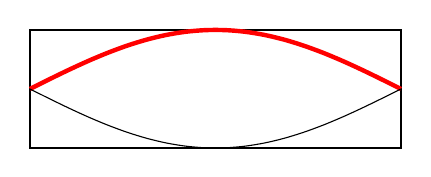
\begin{tikzpicture}[scale=1.5,yscale=.5]
      \draw[thick](0,-1) rectangle(pi,1);
      \draw[smooth,samples=20,domain=0:pi,red,ultra thick]
      plot({\x},{sin(180/pi*\x)});
      \draw[smooth,samples=20,domain=0:pi] plot({\x},{-1*sin(180/pi*\x)});
    \end{tikzpicture}
    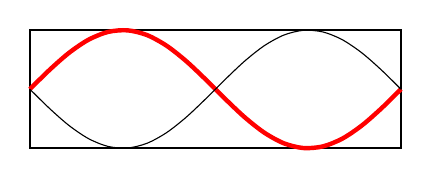
\begin{tikzpicture}[scale=1.5,yscale=.5]
      \draw[thick](0,-1) rectangle(pi,1);
      \draw[smooth,samples=20,domain=0:pi,red,ultra thick]
      plot({\x},{sin(360/pi*\x)});
      \draw[smooth,samples=20,domain=0:pi] plot({\x},{-1*sin(360/pi*\x)});
    \end{tikzpicture}\\
    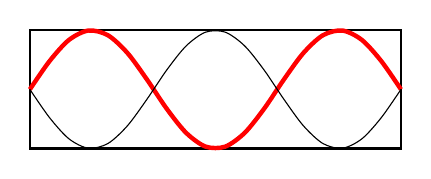
\begin{tikzpicture}[scale=1.5,yscale=.5]
      \draw[thick](0,-1) rectangle(pi,1);
      \draw[smooth,samples=20,domain=0:pi,red,ultra thick]
      plot({\x},{sin(540/pi*\x)});
      \draw[smooth,samples=20,domain=0:pi] plot({\x},{-1*sin(540/pi*\x)});
    \end{tikzpicture}
    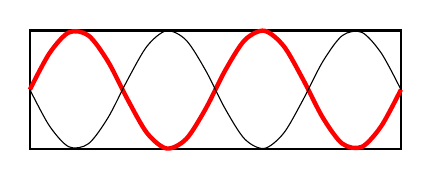
\begin{tikzpicture}[scale=1.5,yscale=.5]
      \draw[thick](0,-1) rectangle(pi,1);
      \draw[smooth,samples=20,domain=0:pi,red,ultra thick]
      plot({\x},{sin(720/pi*\x)});
      \draw[smooth,samples=20,domain=0:pi] plot({\x},{-1*sin(720/pi*\x)});
    \end{tikzpicture}
  \end{center}
  
  No musical instruments are built this way, but you can model standing waves
  inside a concert hall this way.
\end{frame}


\begin{frame}{Standing Waves in Closed Pipes}

  Like strings, pipes that are \emph{closed at both ends} also have a full set
  of harmonics. The $n$-th resonance frequency is given by:
  
  \eq{-.2in}{
    \boxed{f_{r,n}=nf_{r,1}}\quad
    \text{\normalsize (closed pipe)}
  }
  
  where $n$ is a whole-number multiple of the fundamental frequency
  $f_{r\mathrm{res},1}$:

  \eq{-.2in}{
    \boxed{f_{r,1}=\frac{v_s}{2L}}
  }

  The difference between a closed pipe and a string is that the wave speed is
  now the speed of sound $v_s$ inside the pipe.
\end{frame}



\begin{frame}{Standing Waves in Open Pipes}
  \begin{itemize}
  \item Example: Some organ pipes, flute
  \item Both ends of the pipes are anti-nodes
  \end{itemize}
  \begin{center}
    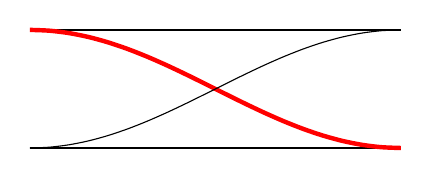
\begin{tikzpicture}[scale=1.5]
      \draw[thick](0,-.5)--(pi,-.5);
      \draw[thick](0,0.5)--(pi,0.5);
      \draw[smooth,samples=20,domain=0:pi,red,ultra thick]
         plot({\x},{0.5*sin(180/pi*\x+90)});
      \draw[smooth,samples=20,domain=0:pi]
        plot({\x},{-.5*sin(180/pi*\x+90)});
    \end{tikzpicture}
    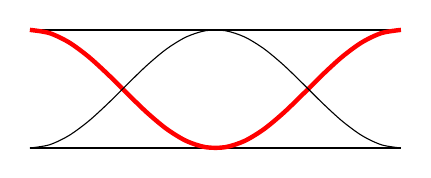
\begin{tikzpicture}[scale=1.5]
      \draw[thick](0,-.5)--(pi,-.5);
      \draw[thick](0,0.5)--(pi,0.5);
      \draw[smooth,samples=20,domain=0:pi,red,ultra thick]
        plot({\x},{0.5*sin(360/pi*\x+90)});
      \draw[smooth,samples=20,domain=0:pi]
        plot({\x},{-.5*sin(360/pi*\x+90)});
    \end{tikzpicture}\\
    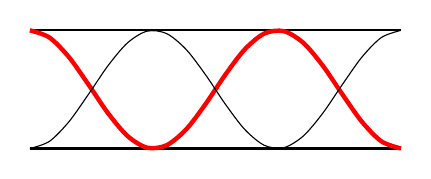
\begin{tikzpicture}[scale=1.5]
      \draw[thick](0,-.5)--(pi,-.5);
      \draw[thick](0,0.5)--(pi,0.5);
      \draw[smooth,samples=20,domain=0:pi,red,ultra thick]
      plot({\x},{0.5*sin(540/pi*\x+90)});
      \draw[smooth,samples=20,domain=0:pi]
      plot({\x},{-.5*sin(540/pi*\x+90)});
    \end{tikzpicture}
    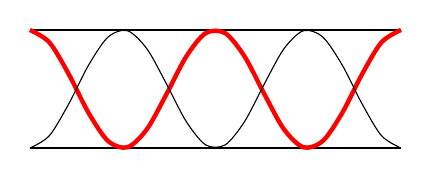
\begin{tikzpicture}[scale=1.5]
      \draw[thick](0,-.5)--(pi,-.5);
      \draw[thick](0,0.5)--(pi,0.5);
      \draw[smooth,samples=20,domain=0:pi,red,ultra thick]
      plot({\x},{0.5*sin(720/pi*\x+90)});
      \draw[smooth,samples=20,domain=0:pi]
      plot({\x},{-.5*sin(720/pi*\x+90)});
    \end{tikzpicture}
  \end{center}
  \begin{columns}
    \column{.5\textwidth}
    First resonance at $\lambda=2L$
    \begin{displaymath}
      f_{r,1}=\frac{v_s}{\lambda}=\frac{v_s}{2L}
    \end{displaymath}
    \column{.5\textwidth}
    Second resonance at $\lambda=L$
    \begin{displaymath}
      f_{r,2}=\frac{v_s}{\lambda}=\frac{v_s}{L}=2f_{r,1}
    \end{displaymath}
  \end{columns}
\end{frame}



\begin{frame}{Standing Waves in Open Pipes}
  Like strings and closed pipes, open pipes also have a
  ``full set of harmonics''. The $n$-th resonance frequency is given by:
  
  \eq{-.2in}{
    \boxed{f_{r,n}=nf_{r,1}}
    \quad\text{\normalsize (open pipe)}
  }
  
  where $n$ is a whole-number multiple of fundamental frequency
  $f_{r,1}$:

  \eq{-.2in}{
    \boxed{f_{r,1}=\frac{v_s}{2L}}
  }

  This is not the case for every configuration. Some common configurations do
  not have a full set of harmonics.
\end{frame}



\begin{frame}{Standing Waves in Semi-Open Pipes}
  \begin{itemize}
  \item Examples: Most organ pipes, clarinet, oboes, brass instruments
  \item Closed end: node (like in the closed pipes)
  \item Open end: anti-node (like in the open pipes)
  \end{itemize}
  \begin{center}
    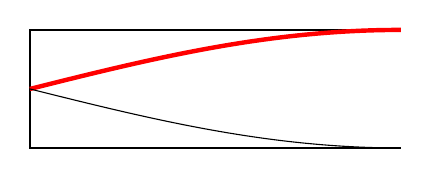
\begin{tikzpicture}[scale=1.5]
      \draw[thick](pi,-.5)--(0,-.5)--(0,.5)--(pi,.5);
      \draw[smooth,samples=20,domain=0:pi,red,ultra thick]
         plot({\x},{0.5*sin(90/pi*\x)});
      \draw[smooth,samples=20,domain=0:pi]
        plot({\x},{-.5*sin(90/pi*\x)});
    \end{tikzpicture}
    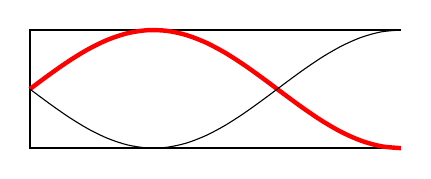
\begin{tikzpicture}[scale=1.5]
      \draw[thick](pi,-.5)--(0,-.5)--(0,.5)--(pi,.5);
      \draw[smooth,samples=20,domain=0:pi,red,ultra thick]
        plot({\x},{0.5*sin(270/pi*\x)});
      \draw[smooth,samples=20,domain=0:pi]
        plot({\x},{-.5*sin(270/pi*\x)});
    \end{tikzpicture}\\
    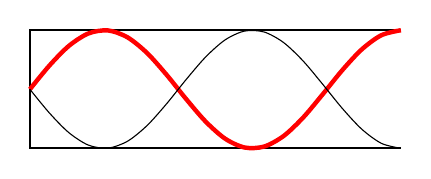
\begin{tikzpicture}[scale=1.5]
      \draw[thick](pi,-.5)--(0,-.5)--(0,.5)--(pi,.5);
      \draw[smooth,samples=20,domain=0:pi,red,ultra thick]
      plot({\x},{0.5*sin(450/pi*\x)});
      \draw[smooth,samples=20,domain=0:pi]
      plot({\x},{-.5*sin(450/pi*\x)});
    \end{tikzpicture}
    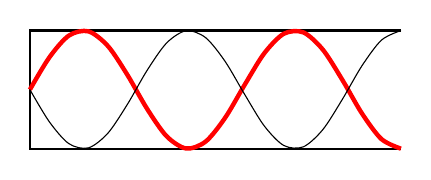
\begin{tikzpicture}[scale=1.5]
      \draw[thick](pi,-.5)--(0,-.5)--(0,.5)--(pi,.5);
      \draw[smooth,samples=20,domain=0:pi,red,ultra thick]
      plot({\x},{0.5*sin(630/pi*\x)});
      \draw[smooth,samples=20,domain=0:pi]
      plot({\x},{-.5*sin(630/pi*\x)});
    \end{tikzpicture}
  \end{center}
\end{frame}



\begin{frame}{Standing Waves in Semi-Open Pipes}
  Again starting with the fundamental frequency (lowest frequency where a
  standing wave can form inside the pipe). This occurs at $\lambda=4L$:

  \vspace{-.1in}
  \begin{center}
    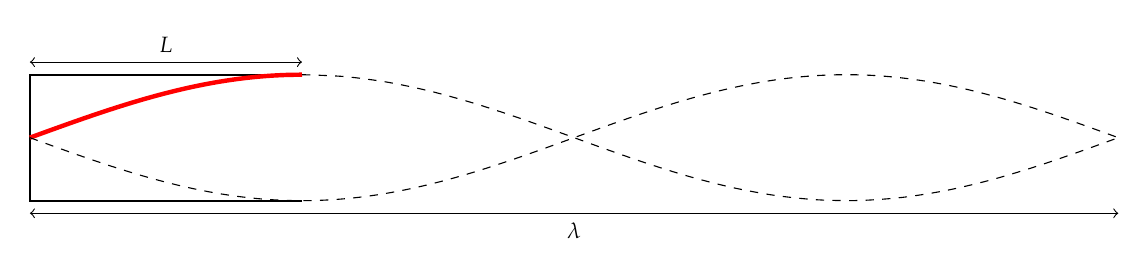
\begin{tikzpicture}[xscale=1.1,yscale=.8]
      \draw[thick](pi,-1)--(0,-1)--(0,1)--(pi,1);
      \draw[smooth,samples=20,domain=0:pi,red,ultra thick]
      plot({\x},{sin(90/pi*\x)});
      \draw[smooth,samples=20,domain=pi:4*pi,dashed]
      plot({\x},{sin(90/pi*\x)});
      \draw[smooth,samples=80,domain=0:4*pi,dashed]
      plot({\x},{-1*sin(90/pi*\x)});
      \draw[<->](0,1.2)--(pi,1.2)
      node[midway,above]{\footnotesize $L$};
      \draw[<->](0,-1.2)--(4*pi,-1.2)
      node[midway,below]{\footnotesize $\lambda$};
    \end{tikzpicture}
  \end{center}
  
  Fundamental frequency $f_{r,1}$ differs from the open-pipe and closed-pipe
  configurations by a factor of $2$:

  \eq{-.2in}{
    \boxed{f_{r,1}=\frac{v_s}{\lambda}=\frac{v_s}{4L}}
  }
\end{frame}



\begin{frame}{Standing Waves in Semi-Open Pipes}
  Likewise, second resonance occurs at
  $\displaystyle \lambda=\frac{4}{3}L$:
  \begin{columns}
    \column{.45\textwidth}
    \centering
    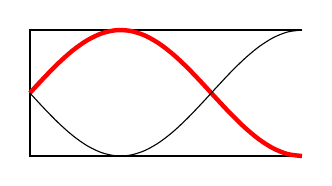
\begin{tikzpicture}[xscale=1.1,yscale=.8]
      \draw[thick](pi,-1)--(0,-1)--(0,1)--(pi,1);
      \draw[smooth,samples=20,domain=0:pi,red,ultra thick]
      plot({\x},{sin(270/pi*\x)});
      \draw[smooth,samples=20,domain=0:pi] plot({\x},{-1*sin(270/pi*\x)});
    \end{tikzpicture}
    
    \column{.55\textwidth}

    \eq{-.4in}{
      f_{r,2}=\frac{v_s}{\lambda}=\frac{3v_s}{4L}=3f_{r,1}
    }
  \end{columns}
  And a third resonance occurs at $\displaystyle \lambda=\frac{4}{5}L$:
  \begin{columns}

    \column{.45\textwidth}
    \centering
    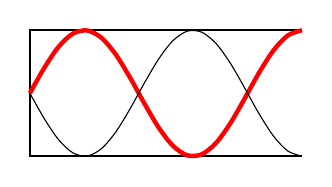
\begin{tikzpicture}[xscale=1.1,yscale=.8]
      \draw[thick](pi,-1)--(0,-1)--(0,1)--(pi,1);
      \draw[smooth,samples=20,domain=0:pi,red,ultra thick]
      plot({\x},{sin(450/pi*\x)});
      \draw[smooth,samples=20,domain=0:pi] plot({\x},{-1*sin(450/pi*\x)});
    \end{tikzpicture}

    \column{.55\textwidth}
    \eq{-.2in}{
      f_{r,3}=\frac{v_s}{\lambda}=\frac{5v_s}{4L}=5f_{r,1}
    }
%    \column{.5\textwidth}
%    \uncover<2->{

%    2nd resonance at $\lambda=\frac{4}{3}L$
%    \uncover<4>{
%    \begin{tikzpicture}[scale=1.2]
%      \draw[thick](pi,-.5)--(0,-.5)--(0,.5)--(pi,.5);
%      \draw[smooth,samples=20,domain=0:pi,red,ultra thick]
%      plot({\x},{0.5*sin(630/pi*\x)});
%      \draw[smooth,samples=20,domain=0:pi]
%      plot({\x},{-.5*sin(630/pi*\x)});
%    \end{tikzpicture}\\
%    4th resonance at $\lambda=\frac{4}{7}L$
%    \begin{displaymath}
%      f_4=\frac{v}{\lambda}=\frac{7v}{4L}=7f_1
%    \end{displaymath}}
  \end{columns}
  
  \vspace{.1in}We can repeat that for $4$th, $5$th\ldots resonances.
\end{frame}



\begin{frame}{Standing Waves in Semi-Open Pipes}
  Only \emph{odd-number multiples} of the fundamental frequency are resonance
  frequencies in a semi-open pipe.  We say that semi-open pipes have an
  \emph{odd} set of harmonics.

  \eq{-.2in}{
    \boxed{f_{r,n} = (2n-1)f_{r,1}}
    \quad\text{\normalsize (semi-open pipes)}
  }
  
  \vspace{-.1in}Because fundamental frequency $f_{r,1}$ is lower than
  open-pipe and closed-pipe configurations by a factor of $2$ for the same
  length $L$, it has advantages when designing organ pipes that produces low
  frequencies.

  \eq{-.2in}{
    \boxed{f_{r,1}=\frac{v_s}{\lambda}=\frac{v_s}{4L}}
  }
\end{frame}


\begin{frame}{Standing Waves in Semi-Open Pipes}
  Remember: harmonic frequencies are multiples of the fundamental frequency.
  This means that:
  \begin{itemize}
  \item 2nd resonance frequency = 3rd harmonic frequency
  \item 3rd resonance frequency = 5th harmonic frequency
  \item 4rd resonance frequency = 7th harmonic frequency
  \end{itemize}
  I mentioned that the \textbf{clarinet} has a wave pattern of this type\ldots
\end{frame}



\begin{frame}{Standing Waves in Semi-Open Pipes}
  \begin{columns}
    \column{.4\textwidth}
    \pic{1}{clarf.png}
    
    \column{.6\textwidth}
    Yes it is! There are no peaks at the even number harmonics!
  \end{columns}
\end{frame}



%\subsection[Res.\ Length]{Resonance Length}
%
%\begin{frame}{Resonance Length in a Semi-Open Pipe}
%  \begin{itemize}
%  \item Now that we have looked at resonance \emph{frequencies}, we'll look
%    at resonance \emph{lengths}
%  \item We produce a \emph{single frequency} in the pipe, and vary the length
%    of the pipe until we have resonance
%  \end{itemize}
%\end{frame}
%
%
%
%\begin{frame}{Resonance Length in a Semi-Open Pipe}
%  Let's submerge a part of this pipe in water. We can change the effective
%  length of the pipe by lowering/raising it.
%  \begin{center}
%    \pic{.5}{images/res-length-closed.png}
%  \end{center}
%
%  \vspace{-.1in}If we place a sound source at the mouth of the pipe (e.g.\
%  tuning fork), at certain lengths, we hear a loud sound coming from the pipe
%\end{frame}
%
%
%\begin{frame}{Resonance Length in a Semi-Open Pipe}
%  The resonance lengths are \emph{odd-number multiples} of the first
%  resonance length $L_{r,1}$: %($\displaystyle\frac{\lambda}{4}$):
%  
%  \eq{-.2in}{
%    \boxed{L_{r,n} = (2n-1)L_{r,1}}
%    \quad\text{\normalsize where}\quad
%    \boxed{L_{r,1} = \frac{\lambda}{4}}
%  }
%\end{frame}
%
%
%
%\begin{frame}{Resonance in an Open Pipe}
%  We can also repeat this with pipes that are open on both ends.
%  \begin{center}
%    \pic{.6}{images/res-length-open.png}
%  \end{center}
%\end{frame}
%
%
%
%\begin{frame}{Resonance in an Open Pipe}
%  Resonance lengths of an open pipe are \emph{whole-number multiples} of the
%  first resonance length $L_{r,1}$:
%
%  \eq{-.25in}{
%    \boxed{L_{r,n}=nL_{r,1}}
%    \quad\text{\normalsize (open pipe)}
%  }
%  
%  \vspace{-.1in}where first resonance length is given by:
%  
%  \eq{-.2in}{
%    \boxed{L_{r,1}=\frac{\lambda}{2}}
%  }
%  
%  This equation looks a lot like the resonance frequency equation. When you
%  read your homework/test questions to make sure you know what the question
%  is asking for.
%\end{frame}
%
%
%
%\begin{frame}{Example Problem}
%  \textbf{Example 5:} A vibrating tuning fork is held near the mouth of a
%  narrow plastic pipe partially submerged in water. The pipe is raised, and the
%  first loud sound is heard when the air column is \SI{9.0}{\centi\metre} long.
%  The temperature in the room is \SI{20}{\celsius}.
%  \begin{itemize}
%  \item Calculate the wavelength of the sound produced by the tuning fork.
%  \item Calculate the length of the air column for the second and third
%    resonances.
%  \item Estimate the frequency of the tune
%  \end{itemize}
%\end{frame}
%
\end{document}
